\documentclass{article}
\usepackage[paperwidth=259pt,paperheight=261pt,margin=0pt,noheadfoot]{geometry}
\usepackage{tikz}
\usetikzlibrary{calc}

\definecolor{ink}{RGB}{28,41,56}
\definecolor{axis}{RGB}{100,116,139}
\definecolor{grid}{RGB}{203,213,225}
\definecolor{curve}{RGB}{30,64,175}
\definecolor{teal}{RGB}{13,148,136}
\definecolor{tealfill}{RGB}{176,227,219}
% Integral diagrams use exactly one semantic palette: blue for the
% lower-only part, yellow for the upper-only (or still unresolved) part, and
% green for their common part.  The common part is explicit rather than an
% alpha blend, so the three meanings stay distinct after GIF quantization.
\definecolor{blue}{RGB}{0,114,178}
\definecolor{bluefill}{RGB}{86,180,233}
\definecolor{yellow}{RGB}{230,159,0}
\definecolor{yellowfill}{RGB}{255,218,102}
\definecolor{green}{RGB}{0,128,84}
\definecolor{greenfill}{RGB}{89,190,142}
\definecolor{orange}{RGB}{234,88,12}
\definecolor{orangefill}{RGB}{254,215,170}
\definecolor{purple}{RGB}{126,34,206}
\definecolor{yellowedge}{RGB}{202,138,4}
\definecolor{projection}{RGB}{148,163,184}
\colorlet{under}{blue}
\colorlet{underfill}{bluefill}
\colorlet{over}{yellow}
\colorlet{overfill}{yellowfill}
\colorlet{shared}{green}
\colorlet{sharedfill}{greenfill}
\colorlet{gap}{yellow}
\colorlet{gapfill}{yellowfill}

\pagestyle{empty}
\setlength\parindent{0pt}
\setlength\topskip{0pt}
\begin{document}
\noindent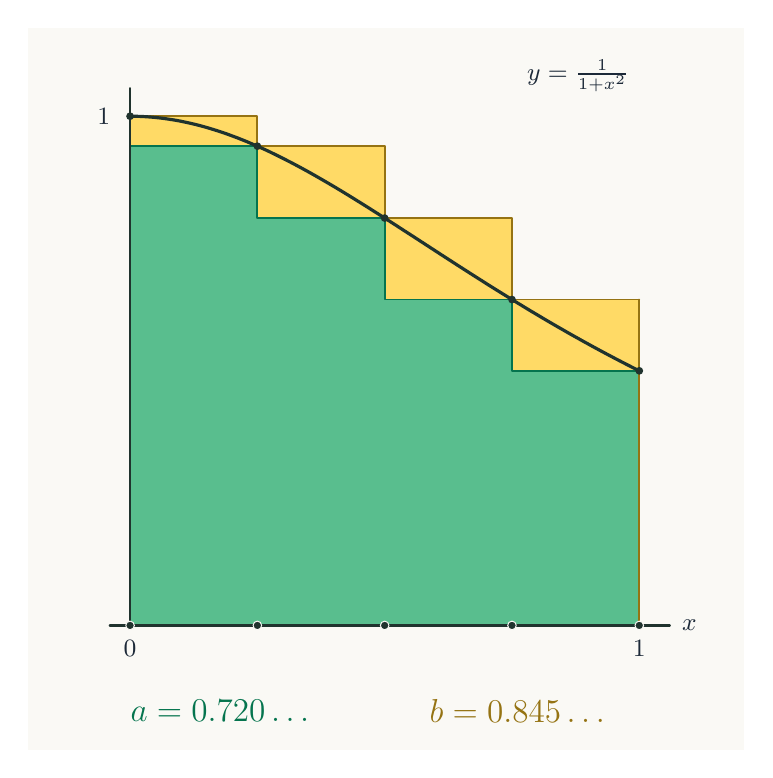
\begin{tikzpicture}[baseline=(current bounding box.north),x=1pt,y=1pt,line cap=round,line join=round]
\useasboundingbox (0,0) rectangle (259,261);
\definecolor{paper}{HTML}{FAF9F5}
\definecolor{graph}{HTML}{20332E}
\colorlet{lowerbound}{shared!85!graph}
\colorlet{upperbound}{yellow!59!graph}
\colorlet{addition}{lowerbound!76!sharedfill}
\colorlet{cutoff}{yellow!85!overfill}
\fill[paper] (0,0) rectangle (259,261);
\begin{scope}[shift={(37,45)},x=184pt,y=184pt]
\fill[overfill] (0,0) -- (0,1) -- (0.25,1) -- (0.25,0.9412) -- (0.5,0.9412) -- (0.5,0.8) -- (0.75,0.8) -- (0.75,0.64) -- (1,0.64) -- (1,0) -- cycle;
\fill[sharedfill] (0,0) -- (0,0.9412) -- (0.25,0.9412) -- (0.25,0.8) -- (0.5,0.8) -- (0.5,0.64) -- (0.75,0.64) -- (0.75,0.5) -- (1,0.5) -- (1,0) -- cycle;
\draw[lowerbound,line width=.65pt] (0,0.9412) -- (0.25,0.9412) -- (0.25,0.8) -- (0.5,0.8) -- (0.5,0.64) -- (0.75,0.64) -- (0.75,0.5) -- (1,0.5);
\draw[upperbound,line width=.65pt] (0,1) -- (0.25,1) -- (0.25,0.9412) -- (0.5,0.9412) -- (0.5,0.8) -- (0.75,0.8) -- (0.75,0.64) -- (1,0.64);
\draw[upperbound,line width=.65pt] (1,0) -- (1,0.64);
\draw[graph,line width=.8pt] (-.04,0) -- (1.06,0);
\draw[graph,line width=.8pt] (0,0) -- (0,1.055);
\draw[graph,line width=1.15pt] plot[smooth] coordinates {(0,1) (0.01,0.9999) (0.02,0.9996) (0.03,0.9991) (0.04,0.9984) (0.05,0.9975) (0.06,0.9964) (0.07,0.9951) (0.08,0.9936) (0.09,0.992) (0.1,0.9901) (0.11,0.988) (0.12,0.9858) (0.13,0.9834) (0.14,0.9808) (0.15,0.978) (0.16,0.975) (0.17,0.9719) (0.18,0.9686) (0.19,0.9652) (0.2,0.9615) (0.21,0.9578) (0.22,0.9538) (0.23,0.9498) (0.24,0.9455) (0.25,0.9412) (0.26,0.9367) (0.27,0.9321) (0.28,0.9273) (0.29,0.9224) (0.3,0.9174) (0.31,0.9123) (0.32,0.9071) (0.33,0.9018) (0.34,0.8964) (0.35,0.8909) (0.36,0.8853) (0.37,0.8796) (0.38,0.8738) (0.39,0.868) (0.4,0.8621) (0.41,0.8561) (0.42,0.8501) (0.43,0.844) (0.44,0.8378) (0.45,0.8316) (0.46,0.8254) (0.47,0.8191) (0.48,0.8127) (0.49,0.8064) (0.5,0.8) (0.51,0.7936) (0.52,0.7872) (0.53,0.7807) (0.54,0.7742) (0.55,0.7678) (0.56,0.7613) (0.57,0.7548) (0.58,0.7483) (0.59,0.7418) (0.6,0.7353) (0.61,0.7288) (0.62,0.7223) (0.63,0.7159) (0.64,0.7094) (0.65,0.703) (0.66,0.6966) (0.67,0.6902) (0.68,0.6838) (0.69,0.6775) (0.7,0.6711) (0.71,0.6648) (0.72,0.6586) (0.73,0.6524) (0.74,0.6462) (0.75,0.64) (0.76,0.6339) (0.77,0.6278) (0.78,0.6217) (0.79,0.6157) (0.8,0.6098) (0.81,0.6038) (0.82,0.5979) (0.83,0.5921) (0.84,0.5863) (0.85,0.5806) (0.86,0.5748) (0.87,0.5692) (0.88,0.5636) (0.89,0.558) (0.9,0.5525) (0.91,0.547) (0.92,0.5416) (0.93,0.5362) (0.94,0.5309) (0.95,0.5256) (0.96,0.5204) (0.97,0.5152) (0.98,0.5101) (0.99,0.505) (1,0.5)};
\node[font=\small,text=ink,anchor=north] at (0,-0.01) {\(0\)};
\node[font=\small,text=ink,anchor=north] at (1,-0.01) {\(1\)};
\node[font=\small,text=ink,anchor=east] at (-0.02,1) {\(1\)};
\node[font=\small,text=ink,anchor=west] at (1.065,0) {\(x\)};
\node[font=\small,text=ink,anchor=east] at (1,1.08) {\(y=\frac{1}{1+x^2}\)};
\filldraw[fill=graph,draw=paper,line width=.35pt] (0,0) circle[radius=1.55pt];
\filldraw[fill=graph,draw=paper,line width=.35pt] (0.25,0) circle[radius=1.55pt];
\filldraw[fill=graph,draw=paper,line width=.35pt] (0.5,0) circle[radius=1.55pt];
\filldraw[fill=graph,draw=paper,line width=.35pt] (0.75,0) circle[radius=1.55pt];
\filldraw[fill=graph,draw=paper,line width=.35pt] (1,0) circle[radius=1.55pt];
\fill[graph] (0,1) circle[radius=1.4pt];
\fill[graph] (0.25,0.9412) circle[radius=1.4pt];
\fill[graph] (0.5,0.8) circle[radius=1.4pt];
\fill[graph] (0.75,0.64) circle[radius=1.4pt];
\fill[graph] (1,0.5) circle[radius=1.4pt];
\end{scope}
\node[anchor=west,inner sep=0pt,text=lowerbound,font=\large] at (37,14) {\(a=0.720\ldots\)};
\node[anchor=west,inner sep=0pt,text=upperbound,font=\large] at (145,14) {\(b=0.845\ldots\)};
\end{tikzpicture}
\end{document}
